\chapter{非线性偏微分方程的精确解及其基础算法}
\section{Introduction}\label{Introduction-01}
In recent years, nonlinear evolution equations (NLEEs) have attracted particular attention from mathematicians, physicists and engineers. There are varieties of methods to construct exact solutions of NLEEs, such as the Inverse Scattering Method \cite{kawata1978inverse,ma2014verifying}, Darboux transformation method \cite{matveev1991darboux,ling2018general,lou1997non}, B{\"a}cklund transformation method \cite{wahlquist1973backlund,li2008method,cheng2015multiple}, Hirota bilinear method \cite{hirota1971exact,hereman1991exact,hu2002application,hirota2003vector,ma2015lump} and Wronskian technique \cite{freeman1983soliton,ito1988reduce,wu2008n}, etc. By using such varieties of schemes, several kinds of exact solutions are obtained, such as solitons \cite{hirota1971exact,makhankov1980computer}, breathers \cite{tajiri1989breather,guo2011rogue,sun2018general}, lump solutions \cite{satsuma1979two,villarroel1999discrete,imai1997dromion}, rogue waves \cite{guo2011rogue,zhang2014rogue,sun2018general,zhaqilao2018symbolic}, and so on.

Hirota bilinear method \cite{hirota1971exact}, which was proposed in 1971, plays an important role in the solving of NLEEs. Especially, the Hirota method is usually applied to construct soliton solutions of NLEEs. With the obtained soliton solutions, we can further calculate breather and lump solutions by the conjugate parameter assignment \cite{tajiri1989breather} and long wave limit \cite{satsuma1979two} method, respectively. These three methods are all algebraic methods to be easily algorithmized and implemented in mathematical softwares, such as, Maple, Mathematica, etc. This paper aims to algorithmize these methods and  implement automated derivation of soliton, breather and lump solutions for (n+1)-dimensional NLEEs.


We should note that the well known formula of n-soliton solution works well for integrable systems, but for non-integrable systems, such as (3+1)KP\CITEcaKP, (3+1)JM\CITEcaJM{} and (3+1)BKP\CITEcaBKP{} equations, it fails. Through a lot of experiments, we found that under appropriate parameters constraints, the false solution (the solution does not meet the original equation) becomes to be genuine solution (the solution meet the original equation). Moreover, the representation of generating formula of m-solitons or m-lumps is not friendly for programming. In order to derive these solutions automatically, these formulas have been properly modified by us in our algorithm for better programming and generalization.

The paper is organized as follows. In \refsec{Method-01}, our algorithm is expounded and an example is given to illustrate the key steps of our algorithm. \refsec{Implementation-01} introduces some details about the implementation and usage of our package. In \refsec{Examples-01}, we apply our program to some examples to illustrate the effectiveness. At the same time, we point out some practical techniques of extending our algorithm to higher dimensional equations. Finally, conclusions are given in \refsec{Conclusions-01}. 

\section{The description  of our algorithm}\label{Method-01}
在我们的算法中, 我们首先利用\Painleve{}分析计算方程的\mk{\Painleve{}截断展开}{从赵银龙的文章里找点内容丰富一下.} (Truncated \Painleve{} Expansion, 简称TPE)\cite{xu2004symbolic,xu2009note}. 以TPE作为变换代入到原方程中, 再用简单Hirota方法计算孤子解. 基于孤子解, 我们通过共轭参数方法得到呼吸子解, 通过长极限方法得到lump解. 

\subsection{The transformation established from truncated \Painleve{} expansion}
对于一个$n+1$维的未知函数$u=u(x_1,\cdots,x_n,t)$, 关于它的NLEE是一个关于$u$及其导数的多项式, 即
\begin{equation}
    U(u,u\up{1},u\up{2},u\up{3}\cdots)=0. \label{oeq}
\end{equation}
其中, $u\up{k}~(k=1,2,3,\cdots)$表示所有的$k$阶导数. 例如, $u\up{1}=\bbrace{u_t,u_{x_1},\cdots,u_{x_n}}$, 以及$u\up{2}=\bbrace{u_{t,x_1},\cdots,u_{t,x_n},u_{x_1,x_2},\cdots}$.

假设原方程存在TPE
\begin{equation}
    u=\frac{1}{f^\alpha}\sum_{k=0}^{\alpha-1}{u_k(x_1,\cdots,x_n,t) f^k}, \label{tr}
\end{equation}
其中 $f=f(x_1,\cdots,x_n,t)$, 而 $\alpha$ 可以通过齐次平衡原则确定 \cite{wang1995solitary,wang1996application}. 一旦确定了$\alpha$的值, 就将\refeqn{tr}代入\refeqn{oeq}, 并令$1/f$的不同次幂的系数为零, 就可以得到关于$u_k~(k=0,\cdots,\alpha-1)$的方程组. 如果关于$u_k~(k=0,\cdots,\alpha-1)$的方程有解, 将其代入\refeqn{tr}就能得到想要的变换; 否则, 整个算法将终止.

事实上, TPE可以看作是对对数变换的推广. 例如, 对数变换$u=R[\ln(f)]_x=R\lfrac{f_x}{f}$和$u=R[\ln(f)]_{xx}=R\sbrace{\lfrac{f_{xx}}{f}-\lfrac{f_x^2}{f^2}}$都满足TPE的形式.

将得到的变换代入\refeqn{oeq}并取分子, 就可以得到关于$f$及其导数的方程, 即
\begin{equation}
    F(f,f\up{1},f\up{2},f\up{3}\cdots)=0. \label{feq}
\end{equation}

\red{展开介绍一下递归求解算法. 简单介绍一下齐次平衡原则的应用. 可以提一下n阶展开方法看下文. 然后那个神奇的例子不知道这里引出来不. 还要点明一点, 从最高次开始求解是为了不求解微分方程.}

\subsection{The simplified Hirota method for constructing soliton solutions}
\red{这里或者绪论中, 需要从Hirota双线性方法到简单Hirota方法过度一下.}

我们利用简单Hirota方法来构造NLEE的孤子解. 需要注意的是, 对于不可积的方程, 直接用简单Hirota方法的m孤子解的公式所生成的孤子解在一定的约束条件下才是原方程的解. 我们的算法对于不可积的方程也是有效的. \mk{}{连接不连贯.}

设$f$是关于行波变量$\xi$的函数, 其中
\begin{equation}
    \xi=p_1\sbrace{x_1+p_2x_2+\cdots+p_nx_n+\omega t}+p_{n+1}. \label{tw}
\end{equation}
这里, $PL=\mbrace{p_1,p_2,\cdots,p_{n+1}}$ 是参数列表. 例如, 当$PL=[k,p,q,c]$时, 
\begin{equation}
    \xi=k(x+py+qz+\omega t)+c.
\end{equation}
将
\begin{equation}
    f=1+\exp\sbrace{\xi} \label{1-soliton}
\end{equation}
代入\refeqn{feq}后可以解得色散关系$\omega$. 

对于一个包含$p_i~(i=1,\cdots,n+1)$的表达式$e$, 我们定义\emph{下标映射函数}
\begin{equation}
    S(e,k): \left\{\begin{array}{ll}
        p_i \rightarrow p_{i,k} & i \in \PS, \\ 
        p_i \rightarrow p_i & i \not\in \PS.
    \end{array}\right.
\end{equation}
其中, $\PS$ 是\emph{参数下标集合}, 且有 
\begin{equation}
    \PS\subseteq  \ALLP=\bbrace{1,2,\cdots,n,n+1}.
\end{equation}
在本文中, $\subseteq$ 表示子集, $\subsetneq$ 表示真子集. 

将
\begin{equation}
    f=1+\exp\sbrace{\xi_i}+\exp\sbrace{\xi_j}+h_{i,j}\exp\sbrace{\xi_i+\xi_j} \label{hij}
\end{equation}
代入\refeqn{feq}后, 可以解得相互作用系数$h_{i,j}$. 这里, $\xi_i=S(\xi,i)$, $\xi_j=S(\xi,j)$.

当$\omega$和$h_{i,j}$都有解时, 我们就可以计算孤子解. 否则, 我们的算法将会结束. 我们称$\omega$和$h_{i,j}$都有解的方程是\emph{可解的}. 否则, 我们称方程是\emph{不可解的}.

需要注意的是, $\PS$在我们的算法中是非常关键的. $\PS= \ALLP$表示算法会根据孤子解的公式生成没有参数约束的解. 本文引入$PS$的理由如下: 
\begin{compactenum}[1. ]
\item 对于一些不可积的方程, 取$\PS= \ALLP$会得到\FalseSol{}. 但是, 取$\PS\subsetneq  \ALLP$会得到\TrueSol{}.
\item 尽管$\PS\subsetneq  \ALLP$能够看作是$\PS= \ALLP$的特例, 但是一些方程会在$\PS= \ALLP$时无法求解$h_{i,j}$.
\item 对于一些不可积的方程, 我们发现让一些$p_{i,k}~(k=1,2,\cdots,m)$ 取值相同就能够得到\TrueSol{}.
\end{compactenum}
在下文中, 我们将以一些具体的例子来说明这些观点. 

Hirota方法中著名的孤子解生成公式是\cite{hirota1973exact}
\begin{equation}
    f_{m-soliton}=\sum_{\mu=0,1}\exp\sbrace{\sum_{i=1}^m{\mu_i \xi_i}+\sum_{1\le i<j\le m}{\mu_i\mu_jH_{i,j}}}. \label{f-soliton-old}
\end{equation}
其中, 求和下标$\mu=0,1$表示对所有可能的取值求和. 事实上, 它的求和范围是$\sbrace{\mu_1,\cdots,\mu_m}\in \bbrace{0,1}^m$. 例如, 
\begin{equation}
\begin{split}
f_{3-soliton}&=1+\exp(\xi_1)+\exp(\xi_2)+\exp(\xi_3)\\
&+h_{1,2}\exp(\xi_1+\xi_2)+h_{2,3}\exp(\xi_2+\xi_3)+h_{1,3}\exp(\xi_1+\xi_3)\\
&+h_{1,2}h_{2,3}h_{1,3}\exp(\xi_1+\xi_2+\xi_3).
\end{split}
\end{equation}
其中, $h_{i,j}=\exp(H_{i,j})$.

这个公式是在Hirota方法的原始文献\cite{hirota1971exact}中以另一种等价形式出现的. 本文中\refeqn{f-soliton-old}的形式是在文献\cite{hirota1973exact}中首次提出的. 这个形式被其他的研究者广泛接受. 但是我们认为\refeqn{f-soliton-old}不利于编程实现. 因此, 我们将其重写为
\begin{equation}
    f_{m-soliton}=\sum_{P\subseteq M}\mbrace{\sbrace{\prod_{\bbrace{i,j}\subseteq P}{h_{i,j}}}\exp\sbrace{\sum_{k\in P}{\xi_k}}}. \label{f-soliton-new}
\end{equation}
其中, $M=\bbrace{1,2,\cdots,m}$, $\xi_k=S(\xi,k)$. 显然, \refeqn{f-soliton-new}和\refeqn{f-soliton-old}是等价的, 并且基于\refeqn{f-soliton-new}进行编程实现更加简单.

\subsection{The conjugate parameter assignment for constructing m-breather solutions}
在得到($2m$)-孤子解后, 我们可以基于共轭参数方法构造对应的$m$-呼吸子解\cite{tajiri1989breather}. 其具体做法如下.

根据文献\cite{tajiri1989breather}, $m$-呼吸子解的生成公式为
\begin{equation}
    f_{m-breather}=\conj{f_{(2m)-soliton}}, \label{f-breather}
\end{equation}
其中${\rm conj}$是一个\emph{共轭参数赋值函数}. 我们有 
\begin{equation}
    p_{i,j}=p_{i,j+m}^*,~(j=1,2,\cdots,m).
\end{equation}
从而, 可以得到$\xi_{j}=\xi_{j+m}^*$. 为了达到上述效果, 我们取
\begin{equation}
\begin{split}
    p_{i,j}&=p_{i,j,RE}+I\cdot p_{i,j,IM}, \\ 
    p_{i,j+m}&=p_{i,j,RE}-I\cdot p_{i,j,IM},
\end{split}
\end{equation}
其中$I$是虚数单位, 而$p_{i,j,RE},p_{i,j,IM}$是实常数. 举一个简单的例子, 取$m=1$, 则1-呼吸子解的生成公式为
\begin{equation}
\begin{split}
f_{1-breather}&=1+\exp(\xi_1)+\exp(\xi_2)+h_{1,2}\exp(\xi_1+\xi_2) \\ 
&=1+\exp(\xi_1)+\exp(\xi_1^*)+h_{1,2}\exp(\xi_1+\xi_1^*).
\end{split}
\end{equation}
由此可以看出, 1-呼吸子解是由2-孤子解导出的. 因此, $m$-呼吸子解能够从$(2m)$-孤子解中导出.

\subsection{The long wave limit method for constructing m-lump solutions}
使用长极限方法\cite{satsuma1979two}, 可以从$(2m)$-孤子解中导出$m$-lump解, 具体步骤如下.

首先, 令
\begin{equation}
\begin{split}
    \xi_i&=k_i\sbrace{x_1+p_ix_2+\cdots+r_ix_n+\omega t}+\xi_i^{(0)},\\
    \eta_i&=\xi_i-\xi_i^{(0)}.
\end{split}
\end{equation}
长极限方法的关键在于当$k_i\rightarrow 0$时, 找到这样两个展开:
\begin{equation}
\begin{split}
    \exp(\eta_i)&=1+k_i \theta_i+o(k_i), \\ 
    h_{i,j}&=1+k_ik_jb_{i,j}+o(k_i^2+k_j^2),
\end{split} \label{lump-expansion}
\end{equation}
其中$o(f)$是Peano余项, 满足$\lim_{f\rightarrow 0}[o(f)/f]=0$.

取$\exp\sbrace{\xi_i^{(0)}}=-1$, 并将\refeqn{lump-expansion} 代入到($2m$)-孤子解的生成公式中, 我们可以得到$m$-lump解. 例如对于一个2-孤子解, 忽略余项后我们有
\begin{equation}
\begin{split}
\Theta_1&=1+\exp(\xi_1)+\exp(\xi_2)+h_{12}\exp(\xi_1+\xi_2) \\ 
&= 1+\exp(\xi_1)+\exp(\xi_2)+(1+k_1k_2b_{12})\exp(\xi_1+\xi_2) \\ 
&=(1+\exp(\xi_1))(1+\exp(\xi_2))+k_1k_2b_{12}\exp(\eta_1+\eta_2) \\ 
&=(1-(1+k_1\theta_1))(1-(1+k_2\theta_2))+k_1k_2b_{12} \\
&=k_1k_2(\theta_1\theta_2+b_{12}).
\end{split}
\end{equation}
因为$k_1k_2$是一个能够被TPE消除的常数因子, 所以1-lump解的公式为
\begin{equation}
    \Theta_1=\theta_1\theta_2+b_{12}.
\end{equation}

根据文献\cite{satsuma1979two}中的证明, 我们可以得到$m$-lump解的生成公式为
\begin{equation}
\begin{split}
    \Theta_m&=\prod_{k=1}^{2m}\theta_k+\frac{1}{2}\sum_{i,j}{b_{i,j}}\prod_{J\neq i,j}{\theta_J}+\frac{1}{2! 2^2}\sum_{i,j,k,l}{b_{i,j}b_{k,l}}\prod_{J\neq i,j,k,l}{\theta_{J}}+\cdots \\
    &+\frac{1}{s!2^s}\sum_{i,j,\cdots,u,v}\underbrace{{b_{i,j}b_{k,l}\cdots b_{u,v}}}_{s}\prod_{J\neq i,j,\cdots, u,v}{\theta_J}+\cdots. \label{f-lump-old}
\end{split}
\end{equation}
例如, 
\begin{equation}
\renewcommand{\t}[1]{\theta_{#1}}
\renewcommand{\b}[1]{b_{#1}}
\begin{split}
\Theta_2&=\t{1}\t{2}\t{3}\t{4}+\b{1,2}\t{3}\t{4}+\b{1,3}\t{2}\t{4}+\b{1,4}\t{2}\t{3}+\b{2,3}\t{1}\t{4}\\
&+\b{2,4}\t{1}\t{3}+\b{3,4}\t{1}\t{2}+\b{1,2}\b{3,4}+\b{1,3}\b{3,4}+\b{1,4}\b{2,3}.
\end{split}
\end{equation}

现在, 我们只需找打\refeqn{lump-expansion}中的展开即可. 将$\eta$看作是一个关于$k$的函数, 我们有  
\begin{equation}
\begin{split}
\exp(\eta(k))&=\exp(\eta(0))+\eta'(0)\exp(\eta(0))k+o(k)\\ 
&=1+\eta'(0)k+o(k). 
\end{split}
\end{equation}
从而, 
\begin{equation}
\theta=\eval{\frac{\partial \eta}{\partial k}}{k=0}=\eval{\frac{\partial \xi}{\partial k}}{k=0}.
\end{equation}
令$h_{i,j}=h(k_i,k_j)$, 根据对称性我们有$h(x,y)=h(y,x)$. 此外, 取$k_2=0$可以将2-孤子解退化为1-孤子解, 所以$h(k_1,0)=1$. 根据对称性, 我们有$h(0,k_2)=1$. 从而, $h(0,0)=1$, 且
\begin{equation}
    h_x(0,0)=\eval{\frac{\partial}{\partial x}h(x,0)}{x=0}=0.
\end{equation}
类似地, 我们有$h_y(0,0)=h_{xx}(0,0)=h_{yy}(0,0)=0$. 因此, $h(x,y)$在$(0,0)$点的展开是 
\begin{equation}
\begin{split}
h(x,y)&=h(0,0)+h_x(0,0)x+h_y(0,0)y \\ 
&+\frac{1}{2}\mbrace{h_{xx}(0,0)x^2+2h_{xy}(0,0)xy+h_{yy}(0,0)y^2}+o(x^2+y^2) \\ 
&=1+h_{xy}(0,0)xy+o(x^2+y^2).
\end{split}
\end{equation}
因此, 我们得到
\begin{equation}
    b_{i,j}=\eval{\frac{\partial^2}{\partial k_i\partial k_j}h_{i,j}}{k_i=0,k_j=0}.
\end{equation}
最终, 对于\refeqn{tw}中的行波变量, lump解的关键参数为
\begin{equation}
\begin{split}
    \theta &= \eval{\frac{\partial \xi}{\partial p_1}}{p_1=0}, \\
    b_{i,j}&= \eval{\frac{\partial^2}{\partial p_{1,i}\partial p_{1,j}}h_{i,j}}{p_{1,i}=0,p_{1,j}=0}.
\end{split} \label{p-lump}
\end{equation}
同时, \refeqn{p-lump}说明有lump解的必要条件是$\bbrace{1}\subsetneq \PS$.

最终, 我们可以基于
\begin{equation}
    f_{m-lump}=\conj{\Theta_m}
\end{equation}
生成$m$-lump解. 然而, 因为\refeqn{f-lump-old}难以理解且不利于变成实现, 我们决定将其重写. 在\refeqn{f-lump-old}中, 如果一个求和项中$b_{i,j}$ 的个数是$s$, 则这个求和项需要除以$s!2^s$. 除以$2^s$表示消除$b_{i,j}=b_{j,i}$的等价情况. 除以$s!$表示消除$b_{i,j}$的全排列.  

基于上述发现, 我们将\refeqn{f-lump-old}重写为
\begin{equation}
    \Theta_m=\sum_{l=0}^m\sum_{s\in L(l)}\sbrace{\prod_{k=1}^l{b_{s_{2k-1},s_{2k}}}\prod_{p\not\in s}{\theta_p}}. \label{f-lump-new}
\end{equation}
其中, 
\begin{equation}
    L(l)=\bbrace{\sbrace{s_1, s_2, \cdots ,s_{2l}}\left|s_{2k}>s_{2k-1},s_{2k+1}>s_{2k-1},s_k\in \bbrace{1,\cdots,2l}\right.}.
\end{equation}
从而, \refeqn{f-lump-new}中的每一个加法项被一个序列$\sbrace{s_1, s_2, \cdots ,s_{2l}}$所唯一确定. 在这个序列中, $s_{2k}>s_{2k-1}$保证了$b_{i,j}=b_{j,i}$的等价情况只出现一次. 类似地, $s_{2k+1}>s_{2k-1}$ 保证了$b_{i,j}$的全排列只出现一次. 

因此, \refeqn{f-lump-new}等价于\refeqn{f-lump-old}, 并且\refeqn{f-lump-new}比\refeqn{f-lump-old}更简单. 并且\refeqn{f-lump-new} 没有冗余的求和项, 从而基于\refeqn{f-lump-new}生成$m$-lump解将比用式 \refeqn{f-lump-old}快.

\red{可以展开一下序列的生成算法.可以展开一下到底快多少倍.}

\subsection{An example of application}
在本节中, 我们将通过一个典型的例子来展示我们的算法是如何工作的.

考虑(3+1)JM方程\CITEcaJM,
\begin{equation}
    u_{xxxy}+3u_{xx}u_y+3u{x}u_{xy}+2u_{ty}-3u_{xz}=0. \label{JMEQ3}
\end{equation}
方程的各项阶数为$\mbrace{\alpha+4,2\alpha+3,2\alpha+3,\alpha+2,\alpha+2}$. 从$\alpha+4=2\alpha+3$可得$\alpha=1$. 因此, 该方程的TPE是$u=u_0/f$. 将其代入到\refeqn{JMEQ3}中, 可以解得$u_0=2f_x$. 从而, \refeqn{JMEQ3}的TPE为 
\begin{equation}
u=\frac{2f_x}{f}. \label{JMEQ-tr}    
\end{equation}

将\refeqn{JMEQ-tr}代入\refeqn{JMEQ3}并取分子, 我们可以得到一个光宇$f$及其导数的方程, 即 
\begin{equation}
\begin{split}
0=&2\,{f}^{2}f_{{{ txy}}}+{f}^{2}f_{{{ xxxxy}}}-3\,{f}^{2}f_{{{ xxz}}}-2\,ff_{{t}}f_{{{ xy}}}-2\,ff_{{{ tx}}}f_{{y}}-2\,ff_{{{ ty}}}f_{{x}}\\
-&4\,ff_{{x}}f_{{{ xxxy}}}+6\,ff_{{x}}f_{{{ xz}}}+3\,ff_{{{ xx}}}f_{{z}}+2\,ff_{{{ xxx}}}f_{{{xy}}}-ff_{{{ xxxx}}}f_{{y}}\\
+&4\,f_{{t}}f_{{x}}f_{{y}}+6\,{f_{{x}}}^{2}f_{{{ xxy}}}-6\,{f_{{x}}}^{2}f_{{z}}-6\,f_{{x}}f_{{{ xx}}}f_{{{ xy}}}+2\,f_{{x}}f_{{{ xxx}}}f_{{y}}. \label{JMEQ-feq}
\end{split}
\end{equation}

取$\xi=k(x+py+qz+\omega t)+c$代入\refeqn{1-soliton}后, 将其结果代入\refeqn{JMEQ-feq}, 可以解得色散关系$\omega=(3q-k^2p)/(2p)$.

令$\PS=\bbrace{1,2}$, 我们有
\begin{equation}
\begin{split}
\xi_i&=k_i\sbrace{x+p_iy+qz+\frac{3q-k_i^2p_i}{2p_i}t}+c, \\ 
\xi_j&=k_j\sbrace{x+p_jy+qz+\frac{3q-k_j^2p_j}{2p_j}t}+c.
\end{split} \label{JMEQ-xij}
\end{equation}
可以看出, 在\refeqn{JMEQ-xij}中, 只有$k$和$p$有下标. 这是由$\PS$指定的. 将\refeqn{JMEQ-xij}代入\refeqn{hij}, 然后将其结果代入\refeqn{JMEQ-feq}, 可以解得相互作用系数为
\begin{equation}
    h_{i,j}=\frac{(k_ip_j(k_i-k_j)+q)p_i^2-p_ip_j(k_jp_j(k_i-k_j)+2q)+qp_j^2}{(k_ip_j(k_i+k_j)+q)p_i^2+p_ip_j(k_jp_j(k_i+k_j)-2q)+qp_j^2}.
\end{equation}
然后, 将\refeqn{p-lump}应用于上述结果, 我们有
\begin{equation}
\begin{split}
&\theta=\frac{2p^2y+(2qz+2x)p+3pq}{2p}, \\ 
&b_{i,j}=-\frac{2p_ip_j(p_i+p_j)}{q(p_i-p_j)}.
\end{split}
\end{equation}

最终, 基于这些中间结果, 我们可以按照下述方法, 分别计算孤子解\zdh 呼吸子解和lump解:
\begin{compactitem}[\textbullet]
\item 将$\omega$和$h_{i,j}$代入\refeqn{f-soliton-new}可以得到孤子解. \reffig{jm:1-soliton}\zdh \reffig{jm:2-soliton}和\reffig{jm:3-soliton}分别展示了1-孤子\zdh 2-孤子和3-孤子解的图像. 
\item 将$\omega$和$h_{i,j}$代入\refeqn{f-breather}可以得到呼吸子解. \reffig{jm:1-breather}\zdh\reffig{jm:2-breather}和\reffig{jm:3-breather}分别展示了1至3阶呼吸子解的图像.
\item 将$\theta$和$b_{i,j}$代入\refeqn{f-lump-new}可以得到lump解. \reffig{jm:1-lump}\zdh\reffig{jm:2-lump}和\reffig{jm:3-lump}分别展示了1至3阶lump解的图像.  
\end{compactitem}

\begin{figure}
\centering 
\subfigure[1-孤子解 \label{jm:1-soliton}]{
    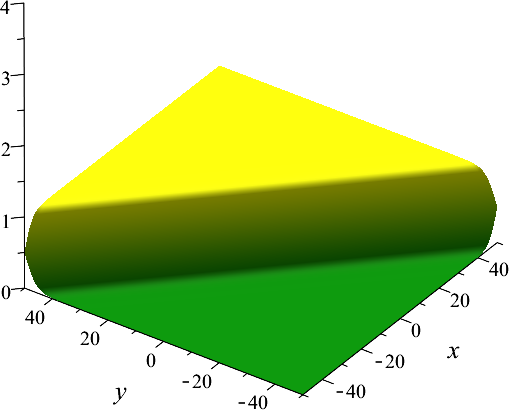
\includegraphics[width=.3\textwidth]{fig/(3+1)JM-1-soliton.png}    
}
\subfigure[2-孤子解 \label{jm:2-soliton}]{
    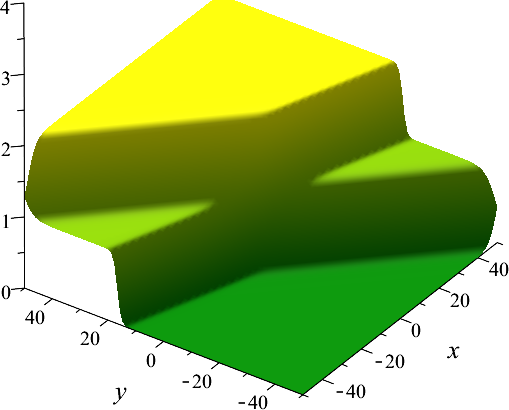
\includegraphics[width=.3\textwidth]{fig/(3+1)JM-2-soliton.png}
}
\subfigure[3-孤子解 \label{jm:3-soliton}]{
    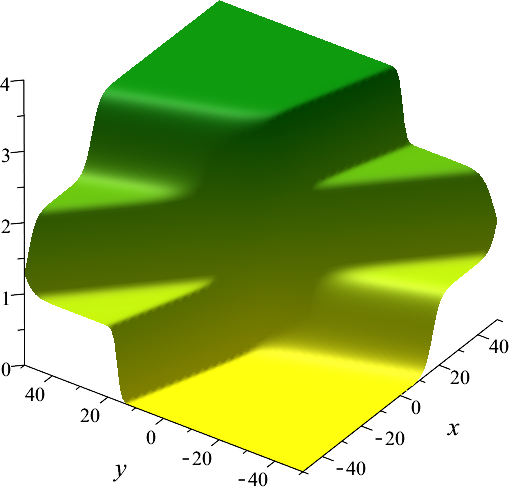
\includegraphics[width=.3\textwidth]{fig/(3+1)JM-3-soliton.png}
}
\subfigure[1-呼吸子解 \label{jm:1-breather}]{
    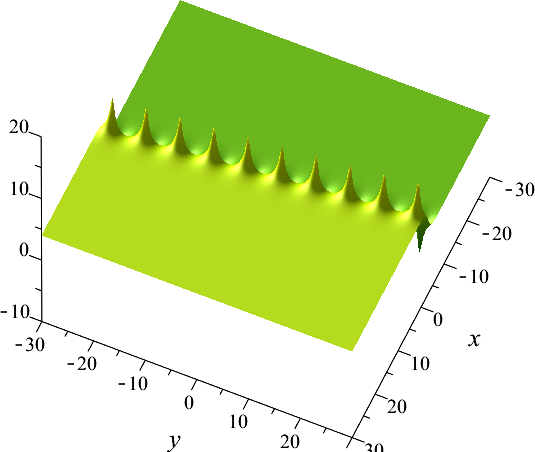
\includegraphics[width=.3\textwidth]{fig/(3+1)JM-1-breather.png}
}
\subfigure[2-呼吸子解 \label{jm:2-breather}]{
    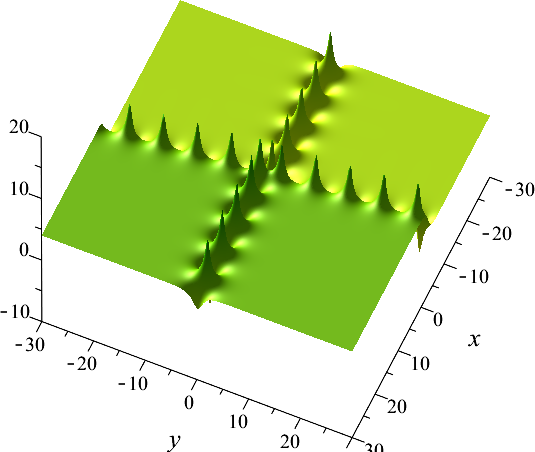
\includegraphics[width=.3\textwidth]{fig/(3+1)JM-2-breather.png}
}
\subfigure[3-呼吸子解 \label{jm:3-breather}]{
    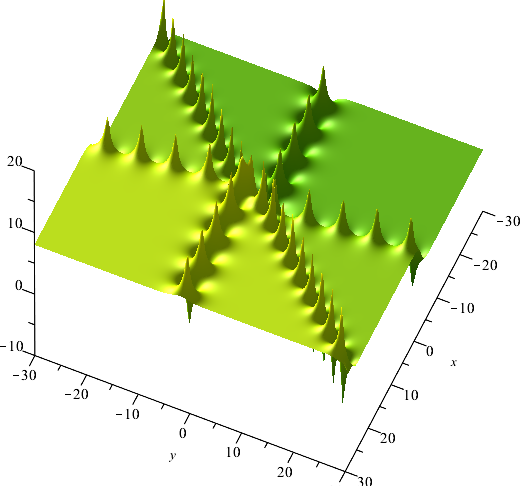
\includegraphics[width=.3\textwidth]{fig/(3+1)JM-3-breather.png}
}
\subfigure[1-lump解 \label{jm:1-lump}]{
    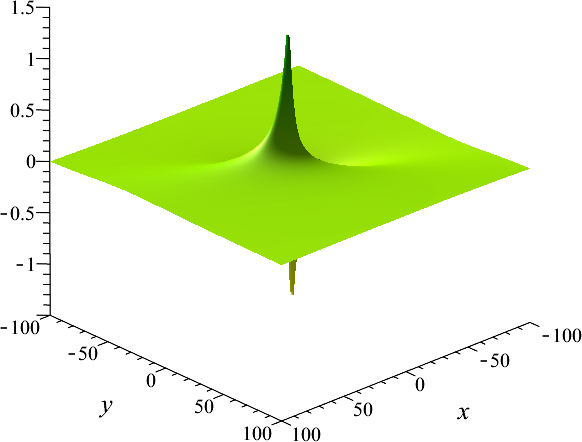
\includegraphics[width=.3\textwidth]{fig/(3+1)JM-1-lump.png}
}
\subfigure[2-lump解 \label{jm:2-lump}]{
    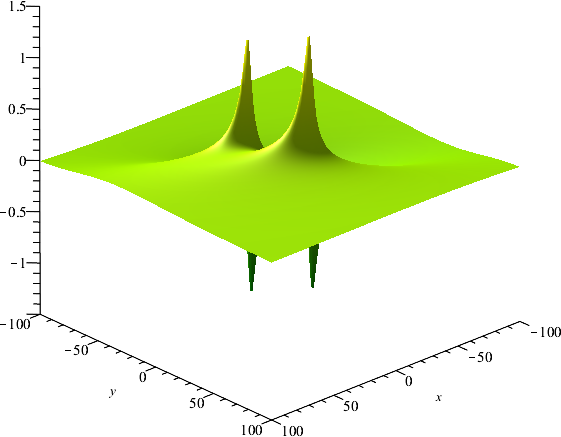
\includegraphics[width=.3\textwidth]{fig/(3+1)JM-2-lump.png}
}
\subfigure[3-lump解 \label{jm:3-lump}]{
    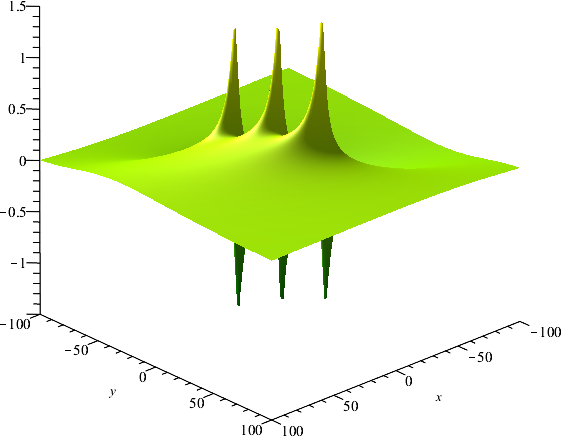
\includegraphics[width=.3\textwidth]{fig/(3+1)JM-3-lump.png}
}
\caption{S(3+1)JM方程的解}
\label{jm}
\end{figure}

有趣的是, 对于1-呼吸子解, 如果关于自变量$x,y$进行画图, 将会得到\reffig{jm:1-breather}. 而关于自变量$x,z$进行画图, 将会得到如\reffig{jm:1-periodic}所示的周期波解. 并且, 对于2-呼吸子解, 若取其中一个呼吸子的参数为实数, 另一个呼吸子的参数仍是复数, 则其图像如\reffig{jm:soliton-breather}所示. 这个可以看做是一个扭状孤子解和一个呼吸子的相互作用解. 

\begin{figure}
\centering
\subfigure[周期波解 \label{jm:1-periodic}]{
    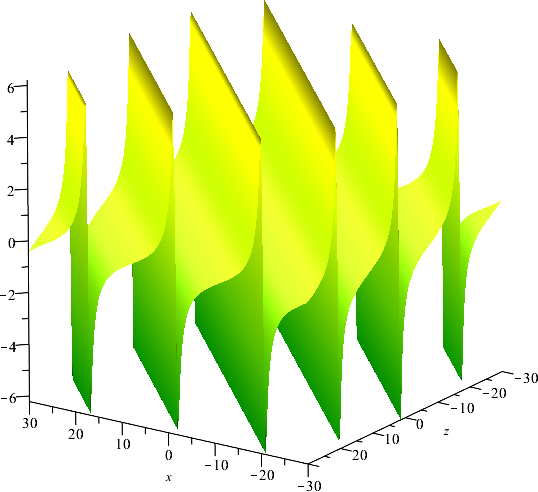
\includegraphics[width=.4\textwidth]{fig/(3+1)JM-1-periodic.png}
}
\subfigure[孤子-呼吸子相互作用解 \label{jm:soliton-breather}]{
    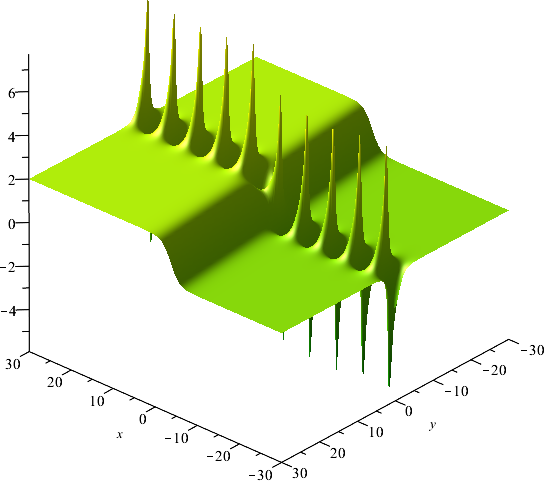
\includegraphics[width=.4\textwidth]{fig/(3+1)JM-soliton-breather.png}
}
\caption{(3+1)JM方程的退化解} \label{jmd}
\end{figure}

\reffig{jm}和\reffig{jmd}的绘图参数如\reftab{jm-plist}所示.

\begin{table}
\centering 
\caption{\reffig{jm}和\reffig{jmd}的绘图参数\label{jm-plist}}
\small
\renewcommand{\arraystretch}{1.1}
\begin{tabular}{cp{0.88\textwidth}}
\hline 
图 & \multicolumn{1}{c}{绘图参数} \\ 
\hline 
\ref{jm:1-soliton} & \texttt{{c=0, q=1, t=0, x=-50..50, y=-50..50, z=0, k[1]=1/2, p[1]=1}} \\
\ref{jm:2-soliton} & \texttt{{c=0, q=1, t=0, x=-50..50, y=-50..50, z=0, k[1]=1/2, k[2]=1/2, p[1]=1, p[2]=3}} \\
\ref{jm:3-soliton} & \texttt{{c=0, q=1, t=0, x=-50..50, y=-50..50, z=0, k[1]=1/2, k[2]=1/2, k[3]=1/2, p[1]=1, p[2]=3, p[3]=1/3}} \\
\ref{jm:1-breather} & \texttt{{c=0, q=1, t=0, x=-30..30, y=-30..30, z=0, k[1,IM]=0, k[1,RE]=1, p[1,IM]=1, p[1,RE]=1/10}} \\
\ref{jm:2-breather} & \texttt{{c=0, q=1, t=0, x=-30..30, y=-30..30, z=0, k[1,IM]=0, k[1,RE]=1, k[2,IM]=1, k[2,RE]=0, p[1,IM]=1, p[1,RE]=1/10, p[2,IM]=1, p[2,RE]=1/10}} \\
\ref{jm:3-breather} & \texttt{{c=0, q=1, t=0, x=-30..30, y=-30..30, z=0, k[1,IM]=0, k[1,RE]=1, k[2,IM]=1, k[2,RE]=0, k[3,IM]=1, k[3,RE]=1, p[1,IM]=1, p[1,RE]=1/10, p[2,IM]=1, p[2,RE]=1/10, p[3,IM]=1, p[3,RE]=1/10}} \\
\ref{jm:1-lump} & \texttt{{q=1, t=0, x=-100..100, y=-100..100, z=0, p[1,IM]=1, p[1,RE]=1}} \\
\ref{jm:2-lump} & \texttt{{q=1, t=0, x=-100..100, y=-100..100, z=0, p[1,IM]=1, p[1,RE]=1, p[2,IM]=1, p[2,RE]=6/5}} \\
\ref{jm:3-lump} & \texttt{{q=1, t=0, x=-100..100, y=-100..100, z=0, p[1,IM]=1, p[1,RE]=1, p[2,IM]=1, p[2,RE]=6/5, p[3,IM]=1, p[3,RE]=4/5}} \\
\ref{jm:1-periodic} & \texttt{{c=0, q=1, t=0, x=-30..30, y=0, z=-30..30, k[1,IM]=1/3, k[1,RE]=0, p[1,IM]=1, p[1,RE]=1/10}} \\
\ref{jm:soliton-breather} & \texttt{{c=0, q=1, t=0, x=-30..30, y=-30..30, z=0, k[1,IM]=1, k[1,RE]=0, k[2,IM]=0, k[2,RE]=1, p[1,IM]=1, p[1,RE]=1/10, p[2,IM]=0, p[2,RE]=1/10}} \\

\hline
\end{tabular}
\end{table}

\section{Implementation and demonstration}\label{Implementation-01}
基于上文的描述, 我们将我们的算法在Maple中实现, 并将其打包在\texttt{TwSolver}中. 在本节中, 我们将简要地介绍我们的程序的接口. 

\texttt{TwSolver}的主要接口是 
\begin{verbatim}
sh:=twsolve(eq,PS,{PL,select_solution}).
\end{verbatim}
其中, \verb|{}|中的参数是可选的. 这些参数的意义如下: 
\begin{compactitem}[\textbullet]
\item \texttt{eq}表示输入方程, 它需要满足\refeqn{oeq}的形式.
\item \texttt{PS}表示\emph{参数下标集合}, 它和$\PS$的意义保持一致. 
\item \texttt{PL}是参数列表, 它和$PL$的意义保持一致.
\item \texttt{select\_solution}是用于控制解的人工选择的参数. 在指定这个参数的情况下, 如果在求解过程中遇到了多解的情况, 程序将会弹出一个对话框让用户选择解. 否则, 程序将默认选择第一个解.
\item 返回值\texttt{sh}是一个\texttt{SolHolder}对象. 它保存了计算的中间结果, 如$\omega,h_{i,j},\theta,b_{i,j}$等. 这些参数能够用于构造孤子解\zdh 呼吸子解和lump解. 
\end{compactitem}
    
例如, 对于(2+1)BKP方程\CITEbaBKP
\begin{equation}
\begin{split}
0&=u_t+u_{xxxxx}-5u_{xxy}-5\int{u_{yy}\dd{x}}+15u_xu_{xx}\\
&+15uu_{xxx}-15uu_y-15u_x\int{u_y\dd{x}}+45u^2u_x, \label{BKP}
\end{split}
\end{equation}
因为它不满足\refeqn{oeq}的形式, 我们不能用\texttt{twsolve}直接求解它. 但是, 令$v=u_x$, 我们有
\begin{equation}
\begin{split}
0&=v_{tx}+v_{xxxxxx}-5v_{xxxy}-5v_{yy}+15v_{xx}v_{xxx}\\
&+15v_xv_{xxxx}-15v_xv_{xy}-15v_{xx}v_y+45v_x^2v_{xx}. \label{BKP-T}
\end{split}
\end{equation}
这是一个能够被我们的程序求解的方程. 调用语句为
\begin{verbatim}
sh:=twsolve(eq,{1,2,3},PL=[k,p,c]).
\end{verbatim}
其中, \texttt{eq}是\refeqn{BKP-T}. 而\texttt{PL=[k,p,c]} 将行波变量指定为$\xi=k(x+py+\omega t)+c$. 如果没有\texttt{PL}, 则默认$\xi=p_1(x+p_2 y+\omega t)+p_3$. 

事实上, 该方程具有2个不同的TPE:
\begin{equation}
v=\frac{2f_x}{f} \text{~~或~~} v=\frac{4f_x}{f}.
\end{equation}
默认情况下, \texttt{select\_solution=false}, 程序会选择$v=2f_x/f$. 而取\texttt{select\_solution=true}之后, 我们将可以任选其中的一个. 调用语句变为
\begin{verbatim}
sh:=twsolve(eq,{1,2,3},PL=[k,p,c],select_solution=true).
\end{verbatim}
在这个例子中, 在对话框中输入1表示选择$v=2f_x/f$. 在这个变换下我们能够求得所有三种类型的解. 但是, 当选择$v=4f_x/f$时, 变换后的方程是\emph{不可解的}. 类似地, 选项\texttt{select\_solution}也能在其它的多解条件下发挥作用.

最终, 该方程的关键参数为
\begin{equation}
\begin{split}
\omega&=-{k}^{4}+5\,{k}^{2}p+5\,{p}^{2}, \\ 
h_{i,j}&=[{k_{{i}}}^{4}-3\,{k_{{i}}}^{3}k_{{j}}+ \left( 4\,{k_{{j}}}^{2}-2\,p_{{i}}-p_{{j}} \right) {k_{{i}}}^{2}-3\,k_{{j}} \left( {k_{{j}}}^{2}-p_{{i}}-p_{{j}} \right) k_{{i}}+{k_{{j}}}^{4}\\
&+\left( -p_{{i}}-2\,p_{{j}}\right) {k_{{j}}}^{2}+ \left( p_{{i}}-p_{{j}} \right) ^{2}]/[{k_{{i}}}^{4}+3\,{k_{{i}}}^{3}k_{{j}}+ \left( 4\,{k_{{j}}}^{2}-2\,p_{{i}}-p_{{j}} \right) {k_{{i}}}^{2}\\
&+3\,k_{{j}} \left( {k_{{j}}}^{2}-p_{{i}}-p_{{j}} \right) k_{{i}}+{k_{{j}}}^{4}+ \left( -p_{{i}}-2\,p_{{j}}\right) {k_{{j}}}^{2}+ \left( p_{{i}}-p_{{j}} \right) ^{2}].
\end{split}
\end{equation}

关于解的一系列操作都基于返回对象\texttt{sh}.  它提供了如下接口: 
\begin{compactitem}[\textbullet]
\item \texttt{sh:-get\_sol(type,m)}能够自动推导类型为type的m阶解. 
\item \verb|sh:-verify_sol(type,m,{s,rnd_assign,method})|用于验证求得的解是否满足原方程. 这里,
\begin{compactitem}[- ]
\item \texttt{s}是参数赋值的集合.
\item 如果指定选项\texttt{rnd\_assign}, 程序将对\texttt{s}中没有赋值的剩余参数进行随机赋值.
\item \texttt{method}用于指定验证解的方法. 我们将在下文中具体介绍这个参数. 
\end{compactitem}
\item \verb|sh:-plot_sol(sol,s)|用于绘制解. 其中
\begin{compactitem}[- ]
\item \texttt{sol} 是一个解. 
\item \texttt{s} 是一个参数赋值的集合. 在绘图时, 所有参数都应该被赋值, 并且需要指定各个自变量的绘图范围.
\end{compactitem}
\end{compactitem}

对于上面的例子, \texttt{sh:-get\_sol(soliton,1)}将会输出绘制(2+1)BKP-T 方程的1-孤子解, 即 
\begin{equation}
v=2\,{\frac {k_{{1}}{{\rm e}^{k_{{1}} \left(  \left( -{k_{{1}}}^{4}+5\,{
k_{{1}}}^{2}p_{{1}}+5\,{p_{{1}}}^{2} \right) t+p_{{1}}y+x \right)+c_1 }}}{
1+{{\rm e}^{k_{{1}} \left(  \left( -{k_{{1}}}^{4}+5\,{k_{{1}}}^{2}p_{{
1}}+5\,{p_{{1}}}^{2} \right) t+p_{{1}}y+x \right)+c_1 }}}}.
\end{equation}

因为验证解的时间要远大于求解的时间, 为了用户的方便, 我们将求解和验证两个过程拆分开来. 在我们的算法中, 2阶以上的孤子解和1阶以上的呼吸子和lump可能不满足原方程. 因此, 我们需要利用\texttt{sh:-verify\_sol(type,m)}来验证他们. 因为对参数赋值后能够极大地提高验证的速度, 我们可以对参数进行人工赋值或者自动赋值. 例如, \texttt{sh:-verify\_sol(soliton,3,rnd\_assign)} 表示对求得的3-孤子解在随机赋值的参数条件下进行验证. 这大概耗时0.06秒. 然而, \texttt{sh:-verify\_sol(soliton,3,$\{k_1=1,k_2=2,k_3=3\}$)}仅对部分参数进行了人工赋值, 它的运行时间约为10秒. 所以, 参数复制能够极大地提高验证解的速度. 

为了进一步提高验证解的速度, 我们考虑了三种不同的验证方法: 
\begin{compactenum}[method-1:]
\item 将变换后的方程的解代入变换后的方程并化简, 并验证指数项的各项系数是否为零.
\item 将变换后的方程的解代入变换后的方程并化简, 并验证其是否为零.
\item 将原方程的解代入原方程并化简, 并验证其是否为零.
\end{compactenum}
\reftab{runtime}中的实验结果表明method-1是最快的方法. 

绘制解解函数的参数和求解以及验证解的函数的参数有所不同. 如果要直接对得到类型为type的m阶解进行绘图, 可以调用\texttt{sh:-plot\_sol([type,m],s)}. 例如, 
\begin{verbatim}
sh:-plot_sol(
    [soliton,1],
    {k[1]=1/4,p[1]=1/5,c[1]=0,t=0,x=-50..50,y=-50..50}
)
\end{verbatim}
可以绘制(2+1)BKP-T方程的1-孤子解. 该解如\reffig{bkp:1-soliton-t}所示, 是一个扭状孤子.

因为$u=v_x$, 如果我们想要绘制(2+1)BKP方程的1-孤子解, 可以用 
\begin{verbatim}
sh:-plot_sol(
    diff(sh:-get_sol(soliton,1),x),
    {k[1]=1/4,p[1]=1/5,c[1]=0,t=0,x=-50..50,y=-50..50}
)
\end{verbatim} 
进行绘制. 该解如\reffig{bkp:1-soliton}所示, 是一个钟状孤子.

此外, \texttt{sh:-plot\_sol}还能接受\texttt{plot3d}的参数来改变绘制结果的外形. 例如, 
\begin{verbatim}
sh:-plot_sol(
    diff(sh:-get_sol(soliton,2),x),
    {k[1]=1/4,p[1]=1/5,k[2]=1/4,p[2]=-2,
    c[1]=0,c[2]=5,x=-50..50,y=-50..50,t=0},
    grid=[400,400],style=surface,axes=frame,
    colorscheme=["zgradient",["Green","Yellow"]]
)
\end{verbatim} 
可以绘制(2+1)BKP方程的2孤子解\refeqn{BKP}. 其图像如\reffig{bkp:2-soliton}所示, 它是由两个钟状孤子相互作用而成的. 并且, 可以看出我们利用\texttt{plot3d}的参数改变了绘制结果的外形.

\begin{figure}[htbp]
\centering
\subfigure[BKP-T方程的1-孤子解 \label{bkp:1-soliton-t}]{
    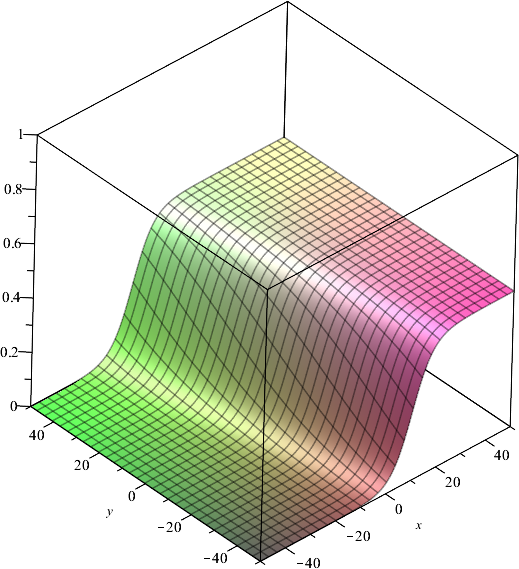
\includegraphics[width=.3\textwidth]{fig/(2+1)BKP-T-1-soliton.png}
}
\subfigure[BKP方程的1-孤子解 \label{bkp:1-soliton}]{
    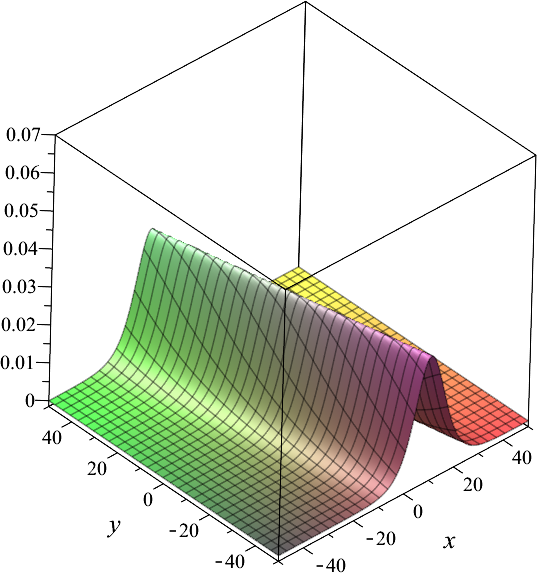
\includegraphics[width=.3\textwidth]{fig/(2+1)BKP-1-soliton.png}
}
\subfigure[BKP方程的2-孤子解 \label{bkp:2-soliton}]{
    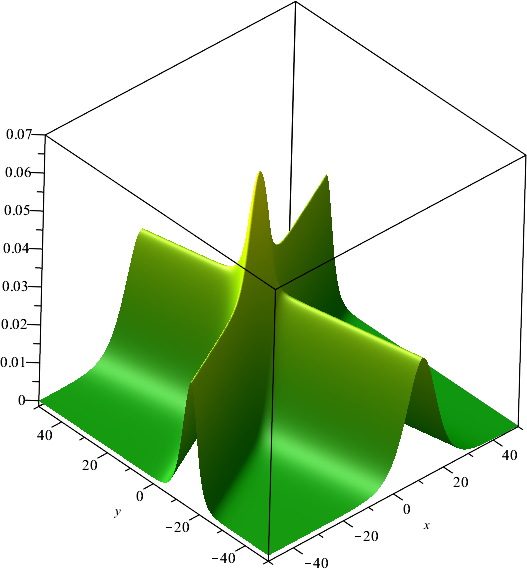
\includegraphics[width=.3\textwidth]{fig/(2+1)BKP-2-soliton.png}
}
\caption{2+1)BKP/BKP-T方程的孤子解}\label{bkp}
\end{figure}

\section{Experiments and examples}\label{Examples-01}
因为$\PS$在我们的算法中起着非常重要的作用, 所以我们选择了一些具有代表性的方程, 在不同的$\PS$取值下对它们进行求解, 来探索$\PS$和方程之间的关系. 实验结果如\reftab{verify}所示.

\begin{table}[htbp]
\centering 
\caption{解的验证结果} \label{verify}
\small
\begin{tabular}{lrcccc}
\hline
\multicolumn{1}{c}{方程名}&\multicolumn{1}{c}{$\PS$} &3-孤子 &2-呼吸子 &2-lump &无解原因\\
\hline
(1+1)KdV &1 &\VTRUE &\VTRUE &- &err-2\\
(2+1)BKP-T &1 &\VTRUE &\VTRUE &- &err-2\\
(2+1)BKP-T &12 &\VTRUE &\VTRUE &\VTRUE &\\
(2+1)CBS &1 &\VTRUE &\VTRUE &- &err-2\\
(2+1)CBS &12 &\VTRUE &\VTRUE &- &err-3\\
(2+1)CBS-G &1 &\VTRUE &\VTRUE &- &err-2\\
(2+1)CBS-G &12 &\VFALSE &\VFALSE &\VFALSE &\\
(2+1)KP &1 &\VTRUE &\VTRUE &- &err-2\\
(2+1)KP &12 &\VTRUE &\VTRUE &\VTRUE &\\
(2+1)SK &1 &\VTRUE &\VTRUE &- &err-2\\
(2+1)SK &12 &\VTRUE &\VTRUE &\VTRUE &\\
(3+1)BKP &1 &\VTRUE &\VTRUE &- &err-2\\
(3+1)BKP &12 &\VTRUE &\VTRUE &\VTRUE &\\
(3+1)BKP &13 &\VTRUE &\VTRUE &\VTRUE &\\
(3+1)BKP &123 &\VFALSE &\VFALSE &\VFALSE &\\
(3+1)CBS &1 &\VTRUE &\VTRUE &- &err-2\\
(3+1)CBS &12 &\VTRUE &\VTRUE &- &err-3\\
(3+1)CBS &13 &\VTRUE &\VTRUE &- &err-3\\
(3+1)CBS &123 &\VTRUE &\VTRUE &- &err-3\\
(3+1)JM &1 &\VTRUE &\VTRUE &- &err-2\\
(3+1)JM &12 &\VTRUE &\VTRUE &\VTRUE &\\
(3+1)JM &13 &\VTRUE &\VTRUE &- &err-3\\
(3+1)JM &123 &\VFALSE &\VFALSE &\VFALSE &\\
(3+1)KP &1 &\VTRUE &\VTRUE &- &err-2\\
(3+1)KP &12 &\VTRUE &\VTRUE &\VTRUE &\\
(3+1)KP &13 &\VTRUE &\VTRUE &\VTRUE &\\
(3+1)KP &123 &\VFALSE &\VFALSE &\VFALSE &\\
(3+1)NEE-T &1 &\VTRUE &\VTRUE &- &err-2\\
(3+1)NEE-T &12 &\VTRUE &\VTRUE &\VTRUE &\\
(3+1)NEE-T &13 &\VTRUE &\VTRUE &- &err-3\\
(3+1)NEE-T &123 &\VFALSE &\VFALSE &\VFALSE &\\
(3+1)YTSF &1 &\VTRUE &\VTRUE &- &err-2\\
(3+1)YTSF &12 &\VTRUE &\VTRUE &\VTRUE &\\
(3+1)YTSF &13 &\VTRUE &\VTRUE &- &err-3\\
(3+1)YTSF &123 &- &- &- &err-1\\
(4+1)Fokas-T &1 &\VTRUE &\VTRUE &- &err-2\\
(4+1)Fokas-T &12 &\VTRUE &\VTRUE &- &err-3\\
(4+1)Fokas-T &13 &\VTRUE &\VTRUE &- &err-3\\
(4+1)Fokas-T &123 &\VFALSE &\VFALSE &\VFALSE &\\
(4+1)Fokas-T-2 &1 &\VTRUE &\VTRUE &- &err-2\\
(4+1)Fokas-T-2 &12 &\VTRUE &\VTRUE &\VTRUE &\\
\hline
\multicolumn{6}{l}{\pbox{0.6\textwidth}{
{\tiny ~}\\
注: err-1表示$h_{i,j}$ 无解, err-2表示lump解需要$\{1\}\subsetneq \PS$, err-3表示0作为除数. 表中出现的方程如果未出现在正文中, 则其表达式在\reftab{eqs}中.
}}
\end{tabular}
\end{table}

\begin{table}[htbp]
\centering
\caption{方程表达式}\label{eqs}
\renewcommand{\arraystretch}{1.2}
\begin{tabular}{lp{0.7\textwidth}}
\hline
\multicolumn{1}{c}{方程名} & \multicolumn{1}{c}{表达式} \\
\hline
(2+1) SK\CITEbaSK & $5\,{u_{{x}}}^{2}u_{{{\it xx}}}+5\,u_{{x}}u_{{{\it xxxx}}}+5\,u_{{x}}u_{{{\it xy}}}+5\,u_{{{\it xx}}}u_{{{\it xxx}}}+5\,u_{{{\it xx}}}u_{{y}}-u_{{{\it tx}}}+u_{{{\it xxxxxx}}}+5\,u_{{{\it xxxy}}}-5\,u_{{{\it yy}}}=0$.\\
(2+1) KP\CITEbaKP & $\alpha\,u_{{{\it yy}}}+6\,uu_{{{\it xx}}}+6\,{u_{{x}}}^{2}+u_{{{\it tx}}}+u_{{{\it xxxx}}}=0$.\\
(2+1) CBS\CITEbaCBS & $4\,u_{{x}}u_{{{\it xy}}}+2\,u_{{{\it xx}}}u_{{y}}+u_{{{\it tx}}}+u_{{{\it xxxy}}}=0$.\\
(2+1) CBS-G\CITEbaCBSG & $\alpha\,u_{{{\it xy}}}+\beta\,u_{{{\it yy}}}+3\,u_{{x}}u_{{{\it xy}}}+3\,u_{{{\it xx}}}u_{{y}}+u_{{{\it tx}}}+u_{{{\it xxxy}}}=0$.\\
(3+1) CBS\CITEcaCBS & $4\,u_{{x}}u_{{{\it xy}}}+4\,u_{{x}}u_{{{\it xz}}}+2\,u_{{{\it xx}}}u_{{y}}+2\,u_{{{\it xx}}}u_{{z}}+u_{{{\it tx}}}+u_{{{\it xxxy}}}+u_{{{\it xxxz}}}=0$.\\
(3+1) BKP\CITEcaBKP & $-3\,u_{{x}}u_{{{\it xy}}}-3\,u_{{{\it xx}}}u_{{y}}+u_{{{\it ty}}}+3\,u_{{{\it xx}}}-u_{{{\it xxxy}}}+3\,u_{{{\it zz}}}=0$.\\
(3+1) KP\CITEcaKP & $-6\,uu_{{{\it xx}}}-6\,{u_{{x}}}^{2}+u_{{{\it tx}}}+u_{{{\it xxxx}}}+3\,u_{{{\it yy}}}+3\,u_{{{\it zz}}}=0$.\\
(3+1) NEE\CITEcaNEE & $3\,u_{{{\it xz}}}-2\,u_{{{\it ty}}}-u_{{{\it xxxy}}}+4\,u_{{x}}u_{{y}}+2\,uu_{{{\it xy}}}+2\,u_{{{\it xx}}}\int \!u_{{y}}\,{\rm d}x=0$.\\
(3+1) NEE-T\CITEcaNEET & $2\,v_{{x}}v_{{{\it xxy}}}+4\,v_{{{\it xx}}}v_{{{\it xy}}}+2\,v_{{{\it xxx}}}v_{{y}}-2\,v_{{{\it txy}}}-v_{{{\it xxxxy}}}+3\,v_{{{\it xxz}}}=0$.\\
(3+1) YTSF\CITEcaYTSF & $3\,\alpha\,u_{{{\it yy}}}+4\,u_{{x}}u_{{{\it xz}}}+2\,u_{{{\it xx}}}u_{{z}}-4\,u_{{{\it tx}}}+u_{{{\it xxxz}}}=0$.\\

\hline
\end{tabular}
\end{table}

In \reftab{verify}, the first column is the name of the considered equation. The postfix `-T' means transformed,  and the postfix `-G' means generalized. The second column is the abbreviation of $\PS$. For example `12' means $\PS=\{1,2\}$. Our tests omit the constant term in the travelling wave variable, because it doesn't affect the verification result.

Since 1-soliton and 2-soliton are solved directly by the undetermined coefficient method, they must meet the original equation. 
It is unnecessary to verify them, so do 1-breather and 1-lump solutions. We need to verify 3-soliton, 2-breather and 2-lump solutions. Here `\VTRUE' means that the solution meets the input equation and `\VFALSE' means that the solution fails. In addition, `-' means that the solution cannot be obtained by our method, and the reason is given in the last column. 

As we can see from \reftab{verify}, for all equations in our test, $\PS=\{1\}$ can generate genuine soliton and breather solutions. 

For most (2+1)-dimensional equations, $\PS= \ALLP$ can generate genuine solutions if it exists except for (2+1)GBS-G equation. (2+1)CBS and (2+1)GBS-G have no lump solution. 

For most (3+1)-dimensional equations in our test, $\PS= \ALLP$ cannot generate genuine soliton solutions, except for the (3+1)CBS equation. For these equations which don't have genuine solutions when $\PS= \ALLP$, have genuine solutions when $\PS=\{1,2\}$ or $\PS=\{1,3\}$. In fact, they have genuine solutions when $(p_i,q_i)~(i=1,2,\cdots)$ are linear dependent.

The (2+1)BKP-T equation and (2+1)NEE-T equation are transformed from the original equation by eliminating integral.  

In addition, dimensionality reduction is also an important technique to extend our method to higher dimensions. The (4+1)Fokas equation \CITEdaFokas{} is a typical example. The expression of this equation is 
\begin{equation}
    u_{tx}-\frac{1}{4}u_{xxxy}+\frac{1}{4}u_{xyyy}+3u_xu_y+3uu_{xy}-\frac{3}{2}u_{wz}=0. \label{Fokas}
\end{equation}
It can be solved directly by our method when $\PS=\{1,3,4\}$. The corresponding TPE is
\begin{equation}
u={\frac {{f_{{x}}}^{2}-{f_{{y}}}^{2}}{{f}^{2}}}+{\frac { \left( -5\,f_{
{{ xx}}}+f_{{{ yy}}} \right) {f_{{x}}}^{2}+8\,f_{{x}}f_{{y}}f_{{
{ xy}}}+{f_{{y}}}^{2} \left( f_{{{ xx}}}-5\,f_{{{ yy}}}
\right) }{5f(f_x^2-f_y^2)}}.
\end{equation}
But calculate the corresponding $\omega$ and $h_{i,j}$ is quite slow. It takes about 90 seconds in our experiment. The time spending on solution verification is unacceptable.

The TPE of this equation is the function w.r.t. $f,f_x$ and $f_y$, we apply the travelling wave transformation $\xi=ax+by$, and get
\begin{equation}
    au_{t\xi}-\frac{a^3b}{4}u_{\xi\xi\xi\xi}+\frac{ab^3}{4}u_{\xi\xi\xi\xi}+3abu_{\xi}^2+3abuu_{\xi\xi}-\frac{3}{2}u_{wz}=0.  \label{Fork-T}
\end{equation}
This equation is denoted as Fokas-T in \reftab{verify}. By reducing to (3+1)-dimension, the  corresponding TPE becomes
\begin{equation}
    u=(a^2-b^2)\sbrace{\frac{f_{\xi}^2}{f^2}-\frac{f_{\xi\xi}}{f}}.
\end{equation}
Assume $\PS=\{1,2,3\}$, we get
\begin{equation}
\begin{split}
    \omega&={\frac {{a}^{3}b{k}^{2}-a{b}^{3}{k}^{2}+6\,pq}{4a}}, \\
    h_{{i,j}}&={\frac {b \left( k_{{i}}-k_{{j}} \right) ^{2}{a}^{3}-{b}^{3}
    \left( k_{{i}}-k_{{j}} \right) ^{2}a-2\, \left( q_{{i}}-q_{{j}}
    \right)  \left( p_{{i}}-p_{{j}} \right) }{b \left( k_{{i}}+k_{{j}}
    \right) ^{2}{a}^{3}-{b}^{3} \left( k_{{i}}+k_{{j}} \right) ^{2}a-2\,
    \left( q_{{i}}-q_{{j}} \right)  \left( p_{{i}}-p_{{j}} \right) }}.
\end{split}
\end{equation}
As we can see from \reftab{verify}, in this case no solution meets the input equation when $\PS=\{1,2,3\}$. But they become genuine solutions when $(p_i,q_i)~(i=1,2,\cdots)$ are linear dependent.

Based on this observation, we apply the transformation $\eta=cw+dz$ to \refeqn{Fork-T}, and get
\begin{equation}
    au_{t\xi}-\frac{a^3b}{4}u_{\xi\xi\xi\xi}+\frac{ab^3}{4}u_{\xi\xi\xi\xi}+3abu_{\xi}^2+3abuu_{\xi\xi}-\frac{3cd}{2}u_{\eta\eta}=0.  \label{Fokas-T-2}
\end{equation}
This equation is denoted as Fokas-T-2 in \reftab{verify}. The key parameters of this equation are
\begin{equation}
\begin{split}
    \omega&={\frac {{a}^{3}b{k}^{2}-a{b}^{3}{k}^{2}+6\,cd{p}^{2}}{4a}}, \\ 
    h_{{i,j}}&={\frac {b \left( k_{{i}}-k_{{j}} \right) ^{2}{a}^{3}-{b}^{3}
    \left( k_{{i}}-k_{{j}} \right) ^{2}a-2\,cd \left( p_{{i}}-p_{{j}}
    \right) ^{2}}{b \left( k_{{i}}+k_{{j}} \right) ^{2}{a}^{3}-{b}^{3}
    \left( k_{{i}}+k_{{j}} \right) ^{2}a-2\,cd \left( p_{{i}}-p_{{j}}
    \right) ^{2}}}.
\end{split}
\end{equation}
As we can see from \reftab{verify}, in this case all obtained solutions meet the input equation.

The runtime of verifying all solutions is summarized in \reftab{runtime}. It can be seen that method-1 is the most efficient in general. The verification of 2-breather solutions takes the most time. So method-1 is the best choice of solution verification. Thus, \texttt{method=1} is the default value in our package. 

\begin{table}[htbp]
\centering 
\caption{运行时间} \label{runtime}
\begin{tabular}{c|ccc|c}
\hline
time(h) &method-1 &method-2 &method-3 &sum\\
\hline
solve &0.002 &0.002 &0.002 &0.005\\
3-soliton &0.002 &0.002 &0.016 &0.020\\
2-breather &0.212 &0.949 &1.551 &2.713\\
2-lump &0.022 &0.022 &0.033 &0.077\\
\hline
sum &0.238 &0.975 &1.602 &2.815\\

\hline
\end{tabular}
\end{table}

\section{Conclusions}\label{Conclusions-01}
Based on the simplified Hirota method, conjugate parameter assignment and long wave limit method, we propose a novel algorithm that can derive possible soliton, breather and lump solutions to NLEEs automatically. For convenience to program and further generalization, we made the following improvements:
\begin{compactitem}[\textbullet]
\item Introduce $\PS$ for getting genuine solutions of non-integrable equations.
\item Infer the computation formula of key parameters for lump solutions in general cases.
\item Rewrite the generate formula of soliton and lump solutions for the convenience to program. 
\end{compactitem}

As the dimension increases, equations usually are non-integrable. In order to get genuine solution by our method, here are some useful techniques:
\begin{compactitem}[\textbullet]
\item Adopt proper subset $\PS\subsetneq  \ALLP$. 
\item Consider linear correlation between parameters.
\item Dimensionality reduction.
\end{compactitem}

Finally, the implemented Maple package \texttt{TwSolver} provides convenient interfaces for solving, verifying and plotting.
